% This is LLNCS.DEM the demonstration file of
% the LaTeX macro package from Springer-Verlag
% for Lecture Notes in Computer Science,
% version 2.4 for LaTeX2e as of 16. April 2010
%
\documentclass[citenumber]{llncs}
%
\usepackage{makeidx}  % allows for indexgeneration
%
\usepackage{hyperref}				% enlaces en el pdf
\hypersetup{colorlinks=true,        % colores en vez de cajas en los enlaces
			linkcolor=blue,         % color of internal links (change box color with linkbordercolor)
    		citecolor=blue,         % color of links to bibliography
    		filecolor=blue,         % color of file links
    		urlcolor=blue}          % color of external links	    

\usepackage{algorithm,algorithmic}
\usepackage{multicol}
\usepackage{graphicx}           	% para manejar imagenes
\usepackage[utf8]{inputenc}

\begin{document}
\mainmatter              % start of the contributions
%
\title{Fast--BR vs. Fast--CT\_EXT Performance Regarding the Density of the Basic Matrix: an Empirical Study	}
%
\titlerunning{Fast--BR vs. CT_EXT}  % abbreviated title (for running head)
%                                     also used for the TOC unless
%                                     \toctitle is used
			 
\author{Vlad\'{i}mir Rodr\'{i}guez-Diez\inst{1,2} \and Jos\'{e}~Fco. Mart\'{i}nez-Trinidad\inst{1}
		 \and J.~Ariel Carrasco-Ochoa\inst{1} \and Manuel~S.~Lazo-Cortés\inst{1}}
%
\authorrunning{Vlad\'{i}mir Rodr\'{i}guez et al.} % abbreviated author list (for running head)
%
%%%% list of authors for the TOC (use if author list has to be modified)
%\tocauthor{Ivar Ekeland, Roger Temam, Jeffrey Dean, David Grove,
%Craig Chambers, Kim B. Bruce, and Elisa Bertino}
%
\institute{Instituto Nacional de Astrof\'{i}sica, \'{O}ptica y Electr\'{o}nica,\\
		   Luis Enrique Erro \# 1, Tonantzintla, Puebla, M\'{e}xico,\\
		   Coordinaci\'{o}n de Ciencias Computacionales,\\
\email{vladimir.rodriguez@inaoep.mx}
\and Universidad de Camag\"{u}ey,\\
	 Circunvalaci\'{o}n Nte. km 5$\frac{1}{2}$, Camag\"{u}ey, Cuba}


\maketitle              % typeset the title of the contribution

\begin{abstract}
	The Testor Theory allows performing feature selection in supervised classification problems. Typical testors are irreducible subsets of features preserving the object discernibility ability of the original set of features. However, finding the complete set of typical testors for a dataset requires a high computational effort.	In this paper, we make an empirical study involving two of the most recent and fastest algorithms of the state of the art: fast--BR and fast--CT\_EXT. Our study is carried out on synthetic basic matrices to control their characteristics. Finally, we evaluate the conclusions drawn from this study over standard datasets from the UCI machine learning repository.

\keywords{Testor Theory, Algorithms, Basic matrix}
\end{abstract}
%
\section{Introduction}
%
	Feature selection is an important task for supervised classification. It consists in identifying those features that provide relevant information for the classification process. Feature selection may improve the efficiency of pattern recognition and machine learning tools without significantly degrading their efficacy.	In the Logical Combinatorial Pattern Recognition~\cite{Martinez2001}, Testor Theory emerges as a solution to feature selection~\cite{Lazo2001,Shulcloper2008}. A testor is a subset of features which allows discerning between objects from different classes by using only its features. A Typical Testor (TT) is defined as a testor which is minimal with respect to inclusion. The main limitation of the Testor Theory is that finding all TTs has exponential complexity regarding the number of attributes in the dataset~\cite{Chikalov13}.
	
	BT and TB algorithms~\cite{Shulcloper1982}, represent one of the first approaches to computing all TTs using the basic matrix. The basic matrix is a reduced representation of the comparison between all pairs of objects belonging to different classes. These algorithms codify a feature subset as a binary word with as many bits as features in the dataset. In this codification, a 1 represents the inclusion of the corresponding feature in the subset. In this way, the candidate subsets are evaluated following the order of the binary numbers, and some candidates are avoided based on the result of previous evaluations over the basic matrix. Several years later, a new algorithm named REC was presented~\cite{Shulcloper1995b}. The main drawback of REC is that it operates directly over the dataset (instead of the	basic matrix), handling a huge amount of superfluous information. With the purpose of resolving this issue, the CER algorithm was created~\cite{Ayaquica1997}, which also introduced a different traversing order for the candidate subsets.
	
	A new traversing order for the candidate subsets was introduced in~\cite{Santiesteban2003} for the LEX algorithm. This new traversing order (which resembles the lexicographical order in which string characters are compared) is used in the most recent and fastest algorithms for computing all TTs. This algorithm introduced also the concept of gap for its pruning process. Once obtained a TT (or a non testor) candidate which includes the last feature in the dataset, the concept of gap allows us to avoid the evaluation of any subset of this candidate. In LEX, the typical condition is verified first and only for those potentially TTs, the testor condition is evaluated. Later, the CT\_EXT algorithm for computing all TTs~\cite{Sanchez2007} was proposed. This algorithm searches for testors without verifying the typical condition, following the traversing order of LEX. This approach, usually leads to a higher number of candidate evaluations, in comparison to LEX. However, the cost of each candidate evaluation is lower. The authors of CT\_EXT show that it is faster than the previous existing algorithm for most datasets. Then, the BR algorithm~\cite{Lias2009} was presented. This new Recursive algorithm based on Binary operations is similar to LEX but its recursive nature encloses a reduction in the number of evaluated candidates. Given a candidate subset, the remaining features (according to the lexicographical order) are tested, and those being rejected are excluded from subsequent evaluations of supersets of the current candidate.
	
	In~\cite{Sanchez2010} a cumulative procedure for the CT\_EXT algorithm was presented. This fast-CT\_EXT implementation, drastically reduces the runtime for most datasets at no extra cost. Then, in~\cite{Lias2013} the gap elimination and column reduction are added to BR, also using binary cumulative operations. The main drawback of fast-BR and BR is, as in LEX, the high cost of evaluating the typical condition for every contributing candidate. 
	
	We have described above the evolution of the so called \emph{external scale} algorithms for typical testor computation. In addition, a different kind of algorithms such as CT~\cite{Bravo83}, CC~\cite{Aguila84} and YYC~\cite{Alba14} has been developed. Algorithms of this kind are called \emph{internal scale} algorithms, and they analyze the distribution of ones into the basic matrix to find out some conditions to guarantee that a subset of attributes is a typical testor. Internal scale algorithms usually evaluate less candidates than external scale algorithms but each candidate evaluation has a higher computational cost. Therefore, the search for fast algorithms for computing typical testors has been biased to external scale algorithms~\cite{Alba14}.
	
	Recently, a thorough study presented in~\cite{Alba13} concluded that no single typical testor finding algorithm have the best performance for any given problem. Other studies~\cite{Lias2013,Rodriguez15}, performed experiments by categorizing the  basic matrices according to the density of 1's they have; i.e. the number of ones divided by the total number of cells of the matrix. Furthermore, in~\cite{Gonzalez15}, the authors highlighted that the number of rows, the density of 1's and the number of typical testors of the basic matrix influence the performance of the algorithms for computing typical testors. With these precedents, in this paper, we present an empirical study to identify a relationship between the density of the basic matrix and the performance of the most successful algorithms: fast--CT\_EXT~\cite{Sanchez2010} and fast--BR~\cite{Lias2013}. From this empirical study, we obtained a simple rule to determine a priory the fastest algorithm for a given dataset. Finally we validate our rule on standard datasets from the UCI dataset repository~\cite{Bache13}. 
	
	We have organized the rest of this paper in the following way. In Section~\ref{basic_conctps}, the theoretical basis for this work are introduced. In Section~\ref{study}, we present our comparative study over synthetic basic matrices and discuss the results. Then, in Section~\ref{evaluation}, the conclusions drawn from the empirical study are validated over standard datasets from the UCI machine learning repository. Finally, in Section~\ref{conclusions}, our conclusions are presented.
%
\section{Basic Concepts} \label{basic_conctps}
%
	In this section, we introduce the main concepts, definitions and propositions supporting the pruning strategies of fast--CT\_EXT and fast--BR. Here, we aim to provide the key elements to understand the differences between these two algorithms. 
	
	Let $DS$ be a dataset with $k$ objects described by $n$ attributes (features) and grouped in $r$ classes. Every attribute in the set of attributes $R=\lbrace x_1,...,x_n \rbrace$, has a predefined boolean comparison criterion. Let $DM$ be the binary comparison matrix obtained from comparing every pair of objects in $DS$ belonging to different classes. Every comparison of a pair of objects adds a row to $DM$ with 0=equal,1=different in the corresponding attribute position (column). $DM$ has $m$ rows and $n$ columns. Comparisons generating a row with only 0's, hereinafter referred to as empty row, imply that two objects from different classes are equal according to their attributes values. 
	
	\begin{definition}\label{def:testor}
		Let $T \subseteq R$ be a subset of attributes from $DS$. We say that T is a testor if in the sub-matrix
		of DM formed by the columns corresponding to attributes in T, there is not any empty row.
	\end{definition} 	
	
	Usually the number of rows in $DM$ ($m$) is large. In~\cite{Lazo2001} a reduction of $DM$ without loss of relevant information is proposed, and it was proved that this reduced matrix, called \textit{basic matrix} ($BM$), and $DM$; have the same set of testors. Then, we can substitute $DM$ by $BM$ in the definition~\ref{def:testor} without any loss of generality. 	
	
	\begin{definition}\label{def:TT}
		A subset of attributes $T \subseteq R$ is a typical testor in BM iff T is a testor and $\forall x_i \in T, T \setminus x_i$ is not a testor. 
	\end{definition}
		
%	
\subsection{Concepts for fast--CT\_EXT}
%
		
	\begin{definition}\label{def:contrib}
		Given $T \subseteq R$ and $x_i \in R$ such that $x_i \notin T$. We say that $x_i$ contributes to T iff the sub-matrix of BM formed with only those attributes in T has more empty rows than that formed with attributes in $T \cup \lbrace x_i \rbrace$.
	\end{definition}	
	
	The core of the CT\_EXT algorithm is supported by propositions~\ref{prop:contrib} and~\ref{prop:superset}; which are stated and proved in~\cite{Sanchez2010} (Theorems 1 and 2 respectively).
	
	\begin{proposition}\label{prop:contrib} 
		Given $T \subseteq R$ and  $x_i \in R$ such that $x_i \notin T$. If $x_i$ does not contribute to T, then 		$T\cup\{x_i\}$ cannot be a subset of any typical testor.
	\end{proposition}

	\begin{proposition}\label{prop:superset} 
		Given $T \subseteq R$ and $Z \subseteq R$ such that $Z \cap T = \emptyset$. If T is a testor, then $T \cup Z$ is a 	testor too, but it is not a typical testor.
	\end{proposition}

%
\subsection{Concepts for fast--BR}
%
	In addition to the propositions exposed above, fast--BR is supported by the following propositions; which are stated and proved in~\cite{Lias2013}.
	
	\begin{definition}\label{def:exclusion}
		Given $T \subseteq R$. We call compatibility mask of $T$, denoted as $cm_T$, to the binary word in which the $j^{\mathit{th}}$ bit is 1 if the $j^{\mathit{th}}$ row of $BM$ has a 1 in only one of the columns corresponding to attributes in $T$, and otherwise it is 0.
	\end{definition}
	
	\begin{proposition}\label{prop:exclude} 
		Given $T \subseteq R$ and $x_i \in R$ such that $x_i \notin T$.	We denote $c_{x_k}$ to the binary word in which the $j^{\mathit{th}}$ bit is 1 if the $j^{\mathit{th}}$ row of $BM$ has a 1 in the column corresponding to $x_k$. If $\exists x_k \in T$ such that $cm_{T \cup \lbrace x_i\rbrace} \wedge c_{x_k}=(0,...,0)$, then, $T \cup \lbrace x_i\rbrace$ cannot be a subset of any typical testor, and we will say that $x_i$ is exclusionary with $T$.
	\end{proposition}
	
	We will refer to Proposition~\ref{prop:exclude} as exclusion evaluation. Proposition~\ref{prop:TT} expresses how to apply the exclusion evaluation for determining whether a subset $T$ of features is a typical testor.
	
	\begin{proposition}\label{prop:TT} 
			Given $T \subseteq R$ and $x_i \in R$ such that $x_i \notin T$. The subset $T \cup \lbrace x_i\rbrace$ is a typical testor iff it is a testor and $x_i$ is not exclusionary with $T$.
	\end{proposition}
		
%
\section{Comparative Study} \label{study}
%
	  From our literature review, we found two families of external scale algorithms: those evaluating first the testor condition and then verifying the typical condition (exclusion evaluation)~\cite{Shulcloper1982,Sanchez2007,Sanchez2010}, and those evaluating the exclusion first and then the testor condition~\cite{Santiesteban2003,Lias2009,Lias2013}. We include in our comparative study the main exponents of these two families: fast--CT\_EXT and fast--BR, respectively. Their candidate evaluation process is illustrated in Fig.~\ref{fig:candeval}.  Since the number of testors is usually a small fraction of the total evaluated candidates, we can state that most of the times fast--BR makes more exclusion evaluations than fast--CT\_EXT. For our experimental study in the next section; we will use, for both algorithms, the implementations provided by their authors\footnote{The source code as well as all the basic matrices and datasets used in our experiments can be downloaded from \url{http://ccc.inaoep.mx/~ariel/CTBRES}}.

	\begin{figure}[htb]
	    \centering
	    \begin{minipage}{.5\textwidth}
	        \centering
	        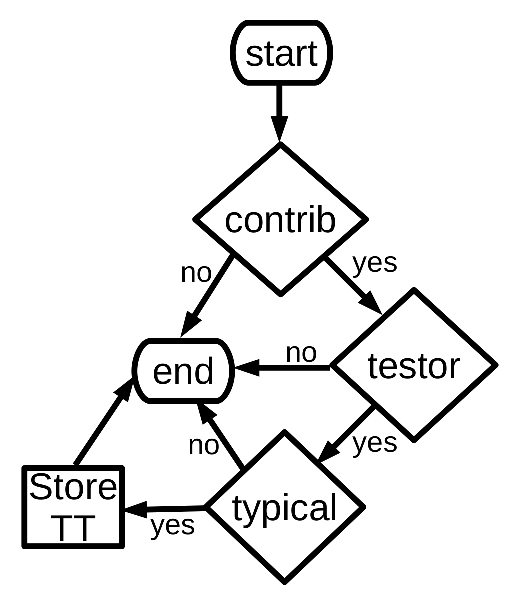
\includegraphics[height=3cm]{ct_ext.eps}
	    \end{minipage}%
	    \begin{minipage}{0.5\textwidth}
	        \centering
	        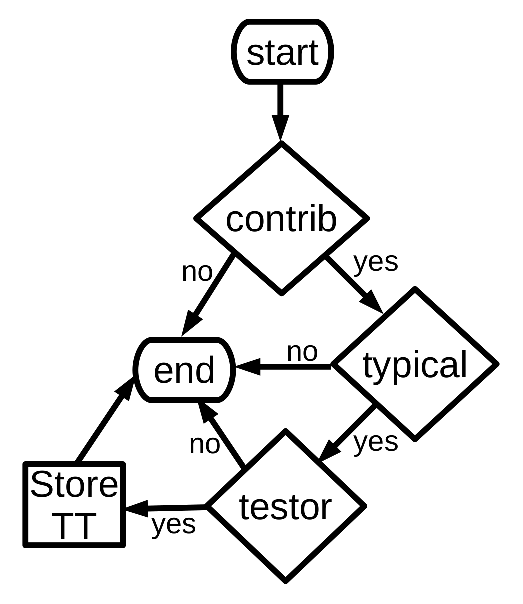
\includegraphics[height=3cm]{BR.eps}	        
	    \end{minipage}
		\caption{Candidate evaluation flowchart for fast--CT\_EXT (left) and fast--BR (right).}
		\label{fig:candeval}
	\end{figure}
	
%
\subsection{Comparison over synthetic basic matrices}
%
	This experiment was designed to explore the influence of the basic matrix density, i.e., the number of ones divided by the total number of cells of the matrix; on the relative performance of fast--CT\_EXT and fast--BR. We conducted this experiment over 500 randomly generated basic matrices with 2000 rows and 30 columns. The size of these matrices was selected in order to keep reasonable runtime for both algorithms. Our 500 matrices were generated with densities of 1's uniformly distributed in the range (0.16--0.80). 

	\begin{figure}[htb]
		\centering
		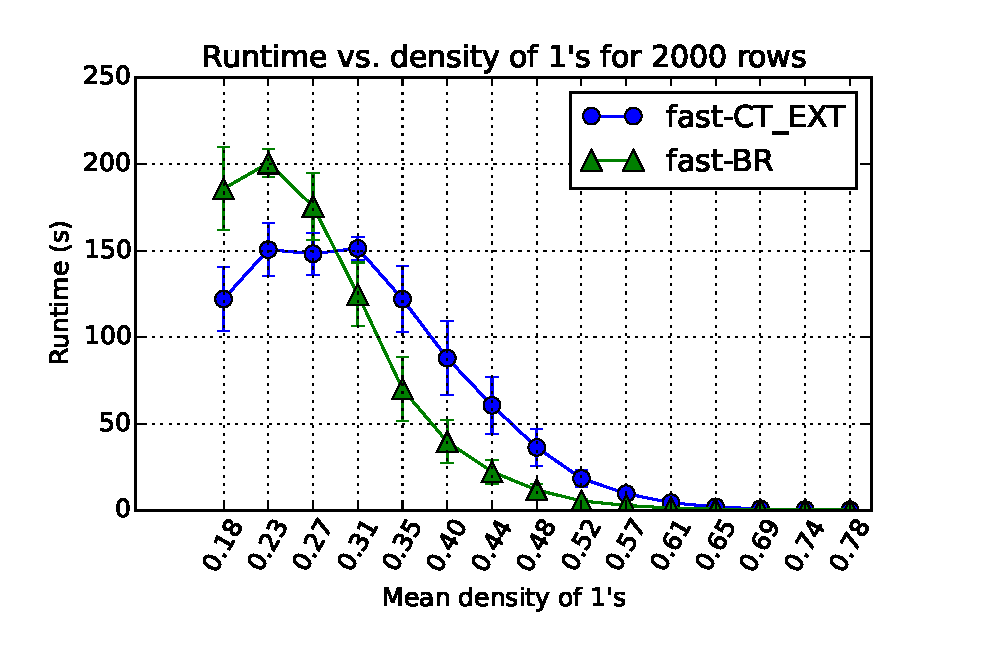
\includegraphics[height=6cm]{2000rows.eps}	        
		\caption{Runtime vs. density for basic matrices with 2000 rows and 30 columns.}
		\label{fig:density}
	\end{figure}

	From Fig.~\ref{fig:density}, it can be seen that fast--CT\_EXT was faster for basic matrices with density under 0.31, while fast--BR was faster for matrices with density above 0.31. A third degree polynomial least square fit to the algorithm's runtime was used to determine their intersection, which was in the density value of 0.31. To understand this behavior, we must look back to Fig.~\ref{fig:candeval}. The exclusion evaluation has the higher computational complexity in both algorithms $\Theta (nm)$. Exclusionary attributes are found when there is at least one column in the basic matrix, considering only those attributes in the current candidate, that can be removed without increasing the number of empty rows. This condition is more frequent in matrices with higher density, where overlapping of 1's is most likely. For matrices with a relative high density, the heavier candidate evaluation process of fast--BR pays off, because exclusionary attributes are avoided from subsequent evaluations. For matrices with lower density, the simpler approach of fast--CT\_EXT results in a faster execution.
	
	For basic matrices with a density value close to the boundary of 0.31, any algorithm can be the fastest; but we may expect a small runtime difference. The overlapping of algorithms' runtime for this region can be seen in  Fig.~\ref{fig:density}. Then, the rule obtained from synthetic matrices may be expressed as: fast--CT\_EXT is faster than fast--BR for basic matrices which have a density of 1's under 0.31, otherwise, fast--BR is faster than fast--CT\_EXT.
%
\section{Evaluation on standard datasets} \label{evaluation}
	In order to evaluate the rule obtained from synthetic basic matrices, we selected 10 datasets from the UCI database repository~\cite{Bache13}. The first four datasets have basic matrix densities clearly under 0.31, the fifth dataset  (mushroom) is close to this value and the last five datasets have densities clearly above 0.31. Numerical attributes were discretized using the Weka's equal width discretization filter with 10 bins, as describe in~\cite{Flores2010}.
	
	\begin{table}[htb]
		\centering \footnotesize
		\caption{Fast--CT\_EXT and fast--BR runtime for standard datasets.}
		\label{tab:density}
		\begin{tabular}{lccccccccc}
			\hline
			\multicolumn{3}{c}{Dataset}& & \multicolumn{2}{c}{Basic Matrix} &&  \multicolumn{1}{c}{Fast--CT\_EXT} & \multicolumn{1}{c}{Fast--BR} \\
			\cline{1-3}\cline{5-6}
			Name   		     & Atts & Instances & & rows  & density  & TTs    & runtime(ms) & runtime(ms) & \%\\
			\hline
			cpu-act			 & 22   & 8192      & & 16    & 0.09     & 6       & \textbf{20} & 35              & 57 \\
			spect-train      & 23   & 80        & & 15    & 0.10     & 26      & \textbf{22} & 29              & 75 \\
			vote             & 17   & 435       & & 15    & 0.11     & 3       & \textbf{2}  & 8               & 25 \\
			pbc              & 19   & 418       & & 45    & 0.24     & 88      & \textbf{28} & 41              & 68 \\
			mushroom         & 23   & 8124      & & 28    & 0.33     & 264     & \textbf{24} & 30              & \textbf{80} \\
			student-por      & 32   & 649       & & 8158  & 0.41     & 851584  & 1874570     & \textbf{161350} & 8  \\
			sponge           & 46   & 76        & & 68    & 0.42     & 10992   & 630         & \textbf{140}    & 22 \\
			student-mat      & 32   & 395       & & 6904  & 0.43     & 679121  & 1003870     & \textbf{81820}  & 8  \\
			lung-cancer      & 57   & 32        & & 237   & 0.47     & 4183355 & 188200      & \textbf{7340}   & 3  \\
			cylinder-bands   & 40   & 512       & & 1147  & 0.55     & 23534   & 5030        & \textbf{530}    & 10 \\
			\hline
		\end{tabular}
	\end{table}
	
	Table~\ref{tab:density} shows the number of attributes and instances for each dataset, the number of rows and the density of the basic matrix, the number of typical testors and the runtime for fast--CT\_EXT and fast--BR. The last column shows the fraction (in percent) of the smallest over the highest runtime for each dataset. Datasets in Table~\ref{tab:density} are sorted by the density of the basic matrix. 
	
	We can see from these results that the rule obtained from synthetic matrices is verified over standard real datasets. Notice that for the mushroom dataset, any algorithm can be the fastest according to our previous study. Indeed, for this particular dataset, the highest runtime fraction was obtained; indicating a similar performance of both algorithms. This fact corroborates our predictions for the boundary region. Another interesting result is that for those datasets with a density clearly above 0.31, fast--BR reached very low runtime fractions. This huge runtime reduction cannot be observed in Fig.~\ref{fig:density}. Thus, we believe that this behaviour is related to the heterogeneous basic matrix dimensions that we have in this experiment. Notice in Table~\ref{tab:density} that the lower ratios in the last column are connected to higher matrix dimensions.
 
%
\section{Conclusions} \label{conclusions}
%
 This paper presents an empirical study on the performance of two algorithms for computing all typical testors, regarding the density of 1's of the basic matrix. We selected for this study the main exponents of two candidate evaluation strategies for external scale algorithms: fast--CT\_EXT and fast--BR. A set of synthetic matrices were used to explore their performance. From our experimental results, we obtained a simple rule for selecting a priori the fastest algorithm for a given dataset. Then, we evaluated this rule over standard datasets from the UCI database repository. We think, however, that the main contribution of this paper is the introduction of a new approach to assess the performance of algorithms for computing typical testors. This approach provides more substantial information than the traditional evaluation over a random sample of datasets.
 
 The evaluation over standard datasets, unveiled higher runtime reductions of fast--BR for basic matrices with larger size. Thus, future work can be directed to study the algorithms' relative performance regarding the number of rows and columns in the basic matrix.
 
%
\section{Acknowledgements} \label{Acknowledgements}
%
	This work was partly supported by National Council of Science and Technology of Mexico under the scholarship grant 399547.

% ---- Bibliography ----
%
\begin{thebibliography}{}
%
% TODO poner los títulos en inglés

\bibitem{Aguila84}	
	Águila, L., Ruíz-Shulcloper, J.  
	Algorithm CC for the elaboration of k-valued information on pattern recognition problems. 
	Mathematics Sciences Journal (In Spanish), 
	5(3) (1984)
	
\bibitem{Alba13}
	Alba-Cabrera, E., Ibarra-Fiallo, J.,Godoy-Calderon, S.:
	A Theoretical and Practical Framework for Assessing the Computational Behavior of Typical Testor-Finding Algorithms.
	In CIARP 2013, Part I. LNCS,
	8258, 351--358, (2013)
	
\bibitem{Alba14}
	Alba-Cabrera, E., Ibarra-Fiallo, J., Godoy-Calderon, S., Cervantes-Alonso, F.:
	YYC: A Fast Performance Incremental Algorithm for Finding Typical Testors.
	Progress in Pattern Recognition, Image Analysis, Computer Vision, and Applications.
	416--423 (2014)
	
\bibitem{Ayaquica1997}
	Ayaquica, I. O.:
	A new external scale algorithm for typical testor computation.
	Memories of the Second Iberoamerican Workshop on Pattern Recognition (In Spanish), 
	Havana, 141--148 (1997)
	
\bibitem{Bache13}	
	Bache, K., Lichman, M.:
	UCI machine learning repository.
	(2013)
	
\bibitem{Bravo83}	
	Bravo-Martínez, A.:
	Algorithm CT for Calculating the Typical Testors of k-valued Matrix. 
	Mathematics Sciences Journal (In Spanish), 
	4(2), 123--144 (1983)
	
\bibitem{Chikalov13}	
	Chikalov, I., Lozin, V. V., Lozina, I., Moshkov, M., Nguyen, H. S., Slowron, A., Zielosko, B.:
 	Three approaches to data analysis. 
 	Springer Science \& Business Media, 
 	(2013)
	
\bibitem{Flores2010}
	Flores, M., G\'{a}mez, J., Mart\'{\i}nez, A. and Puerta, J.:
	Analyzing the impact of the discretization method when comparing Bayesian classifiers.
	Lecture Notes in Computer Science,
	6096 LNAI,  570--579 (2010)

\bibitem{Gonzalez15}		
	González-Guevara, V., Godoy-Calderón, S., Alba-Cabrera, E.,  Ibarra-Fiallo, J.:
	A Mixed Learning Strategy for Finding Typical Testors in Large Datasets. 
	In CIARP 2015. LNCS,
	5197, 716--723 (2008)
		
\bibitem{Lazo2001}	
	Lazo-Cort\'es, M., Ruíz-Shulcloper, J., Alba-Cabrera, E.:
	An Overview of the Evolution of the Concept of Testor. 
	Pattern Recognition. 34, 753--762 (2001)

\bibitem{Lias2009}
	Lias-Rodr\'iguez, A., Pons-Porrata, A.:
	BR: A new method for computing all typical testors. 
	Lecture Notes in Computer Science.
	5856 LNCS, 433--440 (2009)

\bibitem{Lias2013}	
	Lias-Rodr\'iguez, A., Sanchez-D\'iaz, G.:
 	An Algorithm for Computing Typical Testors Based on Elimination of Gaps and Reduction of Columns.
 	International Journal of Pattern Recognition and Artificial Intelligence. 27(08), 1350022 (2013)

\bibitem{Martinez2001}
	Mart\'inez-Trinidad, J.F., Guzm\'an-Arenas, A.: 
	The Logical Combinatorial Approach to Pattern Recognition an Overview through Selected Works. 
	Pattern Recognition. 34, 741--751 (2001)

\bibitem{Rodriguez15}	
	Rodríguez-Diez, V., Martínez-Trinidad, J. F., Carrasco-Ochoa, J. A., Lazo-Cortés, M., Feregrino-Uribe, C., Cumplido, R.:
	A fast hardware software platform for computing irreducible testors. 
	Expert Systems with Applications, 
	42(24), 9612–9619 (2015)

\bibitem{Shulcloper1995b}
	Ruíz-Shulcloper, J., Alba-Cabrera, E., Lazo-Cort\'es, M.:
	Introduction to Typical Testors theory.
	Green Series (In Spanish), No. 50 . CINVESTAV-IPN, México, (1995)
	
\bibitem{Shulcloper1982}	
	Ruíz-Shulcloper, J., Aguila, L., Bravo, A.:
	BT and TB algorithms for computing all irreducible testors. 
	Mathematics Sciences Journal (In Spanish), 2, 11--18 (1982)

\bibitem{Shulcloper2008}
	Ruíz-Shulcloper, J.:
	Pattern recognition with mixed and incomplete data. 
	Pattern Recognition and Image Analysis. 18(4), 563--576 (2008)
	
\bibitem{Sanchez2007}
	Sanchez-D\'iaz, G., Lazo-Cort\'es, M.:
	CT-EXT: an algorithm for computing typical testor set. 
	In Progress in Pattern Recognition, Image Analysis and Applications. 
	Springer. 506--514 (2007)

\bibitem{Sanchez2010}
	Sanchez-D\'iaz, G., Piza-Davila, I., Lazo-Cort\'es, M., Mora-Gonz\'alez, M., Salinas-Luna, J.:
	A fast implementation of the CT-EXT algorithm for the testor property identification. 
	Lecture Notes in Computer Science, 6438 LNAI(PART 2), 92--103 (2010)

\bibitem{Santiesteban2003}	
	Santiesteban, Y., Pons-Porrata, A.:
	LEX: a new algorithm for the calculus of typical testors. 
	Mathematics Sciences Journal (In Spanish), 21(1), 85--95 (2003)
	
	
\end{thebibliography}

%\clearpage
%\addtocmark[2]{Author Index} % additional numbered TOC entry
%\renewcommand{\indexname}{Author Index}
%\printindex
%\clearpage
%\addtocmark[2]{Subject Index} % additional numbered TOC entry
%\markboth{Subject Index}{Subject Index}
%\renewcommand{\indexname}{Subject Index}
%\input{subjidx.ind}
\end{document}
